\documentclass{ximera}
\graphicspath{     %% setup a global graphics path
{./}               %% look in the same-level directory
{./pictures/}      %% look in graphics
{../pictures/}     %% look up one directory, then in graphics
%{../../pictures/} %% look up two directories, then in graphics
}

\author{Zack Reed} %PEter Selinger
\title{Bringing Everything Together: Gauss and Echelon Forms}
\begin{document}
\begin{abstract}
Here we introduce one of the most prevalent applications of matrices and vectors, the solving of systems of equations.
\end{abstract}
\maketitle

\section*{Gaussian Elimination and Rank}
\subsection*{Row Echelon and Reduced Row Echelon Forms}
 
In \href{https://ximera.osu.edu/oerlinalg/LinearAlgebra/SYS-0020/main}{Augmented Matrix Notation and Elementary Row Operations}, we learned to write linear systems in \dfn{augmented matrix} form and use elementary row operations to transform an augmented matrix to \dfn{row-echelon form} and the \dfn{reduced row-echelon form} in order to solve linear systems. 
 
Recall that a matrix (or augmented matrix) is in \dfn{row-echelon form} if:
\begin{itemize}
\item All entries {\it below} each leading entry are $0$.
\item Each leading entry is in a column to the right of the leading entries in the rows above it.
\item All rows of zeros, if there are any, are located below non-zero rows.
\end{itemize}
 
A matrix in row-echelon form is said to be in \dfn{reduced row-echelon form} if it has the following additional properties
\begin{itemize}
\item Each leading entry is a $1$
\item All entries {\it above} each leading $1$ are $0$
\end{itemize}
 
 
Matrices in row-echelon form and reduced row-echelon form are ``convenient" because their corresponding systems of equations are easy to solve. 
 
In this module we turn to the question of existence and uniqueness of the two echelon forms.  Can every matrix (augmented matrix) be carried to a row-echelon form?  If so, is the row-echelon form unique?  Can every matrix be reduced to a reduced row-echelon form?  If so, is the reduced row-echelon form unique?  The answers we find will have long-lasting implications.
 
 
\begin{exploration}\label{init:gaussianelim1}
Solve the following system of equations.
$$\begin{array}{ccccccccc}
      x &+ &2y&-&3z&= &1 \\
     -5x& +&2y&-&3z&=&1\\
      x&- &2y&+&z&=&1
    \end{array}$$
 
We create an augmented matrix corresponding to the system and apply row operations until the matrix is in row-echelon form. 
$$\left[\begin{array}{ccc|c} 
 1&2&-3&1\\-5&2&-3&1\\1&-2&1&1
 \end{array}\right]
 \begin{array}{c}
 \\
 \xrightarrow{R_2+5R_1}\\
 \xrightarrow{R_3-R_1}\\
 \end{array}
\left[\begin{array}{ccc|c} 
 1&2&-3&1\\0&12&-18&6\\0&-4&4&0
 \end{array}\right]
 \begin{array}{c}
 \\
 \\
 \xrightarrow{R_3+\frac{1}{3}R_2}\\
 \end{array}$$
 \begin{equation}\label{eq:ref1}
 \left[\begin{array}{ccc|c} 
 1&2&-3&1\\0&12&-18&6\\0&0&-2&2
 \end{array}\right]
\end{equation}
 
Note that the elementary row operations that lead to (\ref{eq:ref1}) were not prescribed.  We may employ row-operations in a different manner and obtain a different matrix in row-echelon form.  For example, suppose for some reason we had begun by switching the first and third rows.
 
$$\left[\begin{array}{ccc|c} 
 1&2&-3&1\\-5&2&-3&1\\1&-2&1&1
 \end{array}\right]
 \begin{array}{c}
 \\
 \xrightarrow{R_1\leftrightarrow R_3}\\
\\
 \end{array}
\left[\begin{array}{ccc|c} 
 1&-2&1&1\\-5&2&-3&1\\1&2&-3&1
 \end{array}\right]
 \begin{array}{c}
 \\
\\
\\
 \end{array}$$
 
Next we would reduce this matrix to row-echelon form, perhaps in this way:
 
$$\left[\begin{array}{ccc|c} 
 1&-2&1&1\\-5&2&-3&1\\1&2&-3&1
 \end{array}\right]
 \begin{array}{c}
 \\
 \xrightarrow{R_2+5R_1}\\
 \xrightarrow{R_3-R_1}\\
 \end{array}
\left[\begin{array}{ccc|c} 
 1&-2&1&1\\0&-8&2&6\\0&4&-4&0
 \end{array}\right]
 \begin{array}{c}
 \\
 \\
 \xrightarrow{R_3+\frac{1}{2}R_2}\\
 \end{array}
$$
\begin{equation}\label{eq:ref2}
 \left[\begin{array}{ccc|c} 
 1&-2&1&1\\0&-8&2&6\\0&0&-3&3
 \end{array}\right]
\end{equation}
 
The augmented matrices in (\ref{eq:ref1}) and (\ref{eq:ref2}) are clearly not the same, but both are in row-echelon form.
 
If we write the systems of equations corresponding to (\ref{eq:ref1}) and (\ref{eq:ref2}), we can employ back substitution to solve them.  The matrix in (\ref{eq:ref1}) corresponds to
$$\begin{array}{ccccccccc}
      x &+ &2y&-&3z&= &1 \\
     & &12y&-&18z&=&6\\
      &&&&-2z&=&2
    \end{array}$$
     
The matrix in (\ref{eq:ref2}) corresponds to   
$$\begin{array}{ccccccccc}
      x &- &2y&+&z&= &1 \\
     & &-8y&+&2z&=&6\\
      &&&&-3z&=&3
    \end{array}$$
     
Because both systems are equivalent to the original system, it is not surprising that back substitution yields the same solution for both systems.
 
$$x=\answer{0},\quad y=\answer{-1},\quad z=\answer{-1}$$
 
%From the last equation we get $z=-1$. 
%Next, from the second equation we have $12y-18(-1)=6$, which yields $y=-1$.
%Finally, the first equation gives us $x+2(-1)-3(-1)=1$.  Solving for $x$ we get $x=0$. 
%Therefore, the solution to the system is $$x=0, y=-1, z=-1$$
%We arrive at a different matrix in row-echelon form, but back-substitution yields the same solution to the system (you should check this):  $$x=0, y=-1, z=-1$$
\end{exploration}
 
It is clear from Exploration \ref{init:gaussianelim1} that a row-echelon form corresponding to a matrix is not unique.  But what about the reduced row-echelon form?
 
\begin{exploration}\label{init:gaussianelim2} In this problem we revisit the system
$$\begin{array}{ccccccccc}
      x &+ &2y&-&3z&= &1 \\
     -5x& +&2y&-&3z&=&1\\
      x&- &2y&+&z&=&1
    \end{array}$$
     
Following the steps we took to get (\ref{eq:ref1}), but taking the process a little further, we get the reduced row-echelon form.
$$\left[\begin{array}{ccc|c} 
 1&2&-3&1\\-5&2&-3&1\\1&-2&1&1
 \end{array}\right]
 \begin{array}{c}
 \\
 \xrightarrow{R_2+5R_1}\\
 \xrightarrow{R_3-R_1}\\
 \end{array}
\left[\begin{array}{ccc|c} 
 1&2&-3&1\\0&12&-18&6\\0&-4&4&0
 \end{array}\right]
 \begin{array}{c}
 \\
 \\
 \xrightarrow{R_3+\frac{1}{3}R_2}\\
 \end{array}$$
 $$\left[\begin{array}{ccc|c} 
 1&2&-3&1\\0&12&-18&6\\0&0&-2&2
 \end{array}\right]
  \color{blue}
 \begin{array}{c}
 \\
  \xrightarrow{\frac{1}{12}R_2}\\
 \xrightarrow{-\frac{1}{2}R_3}\\
 \end{array}
 \left[\begin{array}{ccc|c} 
 1&2&-3&1\\0&1&-\frac{3}{2}&\frac{1}{2}\\0&0&1&-1
 \end{array}\right]
  \begin{array}{c}
  \xrightarrow{R_1+3R_3}\\
 \xrightarrow{R_2+\frac{3}{2}R_3}\\
\\
 \end{array}$$
\begin{equation}\label{eq:rref3}  \color{blue}
 \left[\begin{array}{ccc|c} 
 1&2&0&-2\\0&1&0&-1\\0&0&1&-1
 \end{array}\right]
  \begin{array}{c}
  \xrightarrow{R_1-2R_2}\\
 \\
\\
 \end{array}
 \color{black}
  \left[\begin{array}{ccc|c} 
 1&0&0&0\\0&1&0&-1\\0&0&1&-1
 \end{array}\right]\end{equation}
Do you think it is possible to start with (\ref{eq:ref2}) and obtain the same reduced row-echelon form?  Try to justify your response.  If possible, find the elementary row operations that take (\ref{eq:ref2}) to the reduced row-echelon form in (\ref{eq:rref3}).
 
$$\left[\begin{array}{ccc|c} 
 1&2&-3&1\\-5&2&-3&1\\1&-2&1&1
 \end{array}\right]
 \begin{array}{c}
 \\
 \xrightarrow{R_1\leftrightarrow R_3}\\
\\
 \end{array}
\left[\begin{array}{ccc|c} 
 1&-2&1&1\\-5&2&-3&1\\1&2&-3&1
 \end{array}\right]$$
$$\begin{array}{c}
 \\
 \xrightarrow{R_2+5R_1}\\
 \xrightarrow{R_3-R_1}\\
 \end{array}
\left[\begin{array}{ccc|c} 
 1&-2&1&1\\0&-8&2&6\\0&4&-4&0
 \end{array}\right]
 \begin{array}{c}
 \\
 \\
 \xrightarrow{R_3+\frac{1}{2}R_2}\\
 \end{array}
$$
\begin{equation*}
  \left[\begin{array}{ccc|c} 
 1&-2&1&1\\0&-8&2&6\\0&0&-3&3
 \end{array}\right]
 \color{red}
 \begin{array}{c}
\rightsquigarrow\text{Elementary}\rightsquigarrow\\
\text{Row Ops.}
\end{array}
 \color{black}
  \left[\begin{array}{ccc|c} 
 1&0&0&0\\0&1&0&-1\\0&0&1&-1
 \end{array}\right]
\end{equation*}
You will be asked to fill in the elementary row operations in Practice Problem \ref{prob:same_rref}.
\end{exploration}
 
Our observations in Exploration \ref{init:gaussianelim2} are summarized in the following diagram.
 
\begin{center}
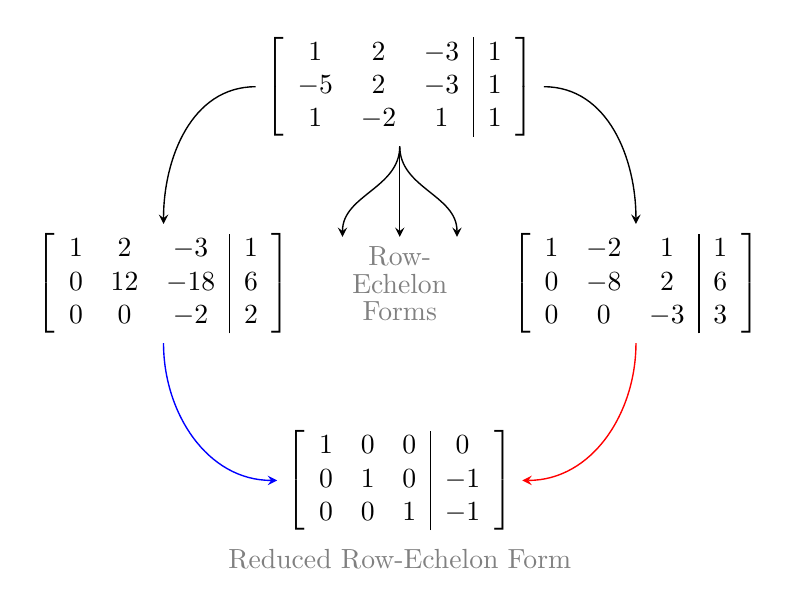
\begin{tikzpicture}
  \node[] at (0, 0)  (o)    {$\left[\begin{array}{ccc|c} 
 1&2&-3&1\\-5&2&-3&1\\1&-2&1&1
 \end{array}\right]$};
 \node[] at (-3, -2.5)  (left1)    {$\left[\begin{array}{ccc|c} 
 1&2&-3&1\\0&12&-18&6\\0&0&-2&2
 \end{array}\right]$};
 \node[] at (3, -2.5)  (right1)    {$\left[\begin{array}{ccc|c} 
 1&-2&1&1\\0&-8&2&6\\0&0&-3&3
 \end{array}\right]$};
 \node[gray] at (0, -2.5)  (c1)    {\shortstack{Row-\\Echelon\\Forms}};
 \node[] at (0, -5)  (c2)    {$\left[\begin{array}{ccc|c}  1&0&0&0\\0&1&0&-1\\0&0&1&-1
 \end{array}\right]$};
 \node[gray] at (0, -6)  (c3)    {Reduced Row-Echelon Form};
  
 \draw [->,line width=0.5pt,-stealth]  (o.west)to[out=180, in=90](left1.north);
  \draw [->,line width=0.5pt,-stealth]  (o.south)to[out=270, in=90](c1.north west);
  \draw [->,line width=0.5pt,-stealth]  (o.south)to[out=270, in=90](c1.north east);
  \draw [->,line width=0.5pt,-stealth]  (o.south)to[out=270, in=90](c1.north);
 \draw [->,line width=0.5pt,-stealth]  (o.east)to[out=0, in=90](right1.north);
 \draw [->,line width=0.5pt,-stealth,blue]  (left1.south)to[out=270, in=180](c2.west);
 \draw [->,line width=0.5pt,-stealth,red]  (right1.south)to[out=270, in=0](c2.east);
 \end{tikzpicture}
 \end{center}
We observed that a row-echelon form associated with a matrix is not unique.  In contrast, we also saw how different sequences of elementary row operations lead to the same solution set and the same reduced row-echelon form.  It turns out that the reduced row-echelon form of a matrix is unique. 


 
\begin{theorem}\label{th:uniquenessofrref} The reduced row-echelon form of a matrix is unique.
\end{theorem}
A proof of this result can be found in [Yuster].
 
The reduced row-echelon form of a matrix is an instance of a row-echelon form of the matrix.  While a given matrix may have multiple row-echelon forms, all row-echelon forms will share one characteristic: the number of nonzero rows in a row-echelon form of the given matrix will be the same.
We will prove this result in Theorem \ref{th:samenumberofnonzerorows}.
 
\section*{Gaussian and Gauss-Jordan Elimination}
 
\begin{definition}[Gaussian Elimination]\label{def:GaussianElimination}
The process of using the elementary row operations on a matrix to transform it into row-echelon form is called \dfn{Gaussian Elimination}.
\end{definition}
 
As we saw in the previous section, it is possible to follow different sequences of row operations to arrive at various row-echelon forms.  However, it was not clear whether it is {\it always possible} to find a row-echelon form.  The following algorithm takes any matrix (or augmented matrix) and transforms it into row-echelon form:
\begin{algorithm}[Gaussian Algorithm] \label{alg:gaussian}
Let $A$ be an $m\times n$ matrix.

 
Set $i=1$ initially.
\begin{itemize}
\item[] Step 1. If $A$ consists entirely of zeros, stop;  $A$ is already in row-echelon form.
 
\item[] Step 2. Otherwise, find the first column from the left containing a nonzero entry in row $i$ or below row $i$.  This column will be called a \dfn{pivot column}.  Go down the pivot column, beginning with row $i$. Pick the topmost nonzero entry and call it $a$. If $a$ is not in row $i$, switch rows so that $a$ moves to row $i$.  Now $a$ is the \dfn{leading entry} in its row.  We will also refer to $a$ as a \dfn{pivot}. 
 
\item[] Step 3. By subtracting multiples of the row containing $a$ from rows below it, make each entry below $a$ zero.
 
\item[] Step 4.  Set $i=i+1$.  If $i > m$ then stop; $A$ is in row-echelon form.
 
\end{itemize}
 
Repeat steps 1--4 on the matrix consisting of the remaining rows.
When the process stops, $A$ will be in row echelon form.
\end{algorithm}
Gaussian Algorithm guarantees that every matrix will have a row-echelon form. 


 
\begin{example}\label{ex:non-augmented}
 
Use the Gaussian Algorithm to find a row-echelon form of $A$ if $$A=\begin{bmatrix}2&4\\1&2\\-1&1\\3&5\end{bmatrix}$$
\begin{explanation}
Following Step 2, we choose the first entry, $2$, as our pivot.  We then perform step 3, using the top row to get zeros in all entries below the $2$.
$$\begin{bmatrix} \fbox{$2$}&4\\1&2\\-1&1\\3&5\end{bmatrix}
  \begin{array}{c}
  \\
  \xrightarrow{R_2-(1/2)R_1}\\
  \xrightarrow{R_3+(1/2)R_1}\\
 \xrightarrow{R_4-(3/2)R_1}\\
 \end{array}
\begin{bmatrix}2&4\\0&0\\0&3\\0&-1\end{bmatrix}
$$
The first row is now complete, and we repeat the process on the rows below it. We identify $3$ as a pivot entry in the second column and move the row containing $3$ to be directly below the first completed row.  We then use the $3$ to make each entry below the $3$ a zero. 
 
$$\begin{bmatrix}2&4\\0&0\\0&\fbox{$3$}\\0&-1\end{bmatrix}
\xrightarrow{R_2\leftrightarrow R_3}\\
\begin{bmatrix}2&4\\0&\fbox{$3$}\\0&0\\0&-1\end{bmatrix}
  \begin{array}{c}
 \\
\\
  \\
 \xrightarrow{R_4+\frac{1}{3}R_2}\\
 \end{array}
 \begin{bmatrix}2&4\\0&3\\0&0\\0&0\end{bmatrix}
$$
This time the algorithm terminates since row 3 and row 4 are zero rows.
\end{explanation}
\end{example}
 
\begin{definition}[Gauss-Jordan Elimination]\label{def:GaussJordanElimination}
The process of using the elementary row operations on a matrix to transform it into reduced row-echelon form is called \dfn{Gauss-Jordan elimination}.
\end{definition}
 
Given a matrix in row-echelon form, it is easy to bring it the reduced row-echelon form.  For example, continuing with Example \ref{ex:non-augmented}, we can start where we left off and compute $\mbox{rref}(A)$.  From our earlier computations we have:
 
$$\begin{bmatrix}2&4\\-1&1\\3&5\\1&2\end{bmatrix}\rightsquigarrow\begin{bmatrix}2&4\\0&3\\0&0\\0&0\end{bmatrix}$$
 
Now we create leading $1's$ and use them to to wipe out all non-zero entries above them.
$$\begin{bmatrix}2&4\\0&3\\0&0\\0&0\end{bmatrix}
  \begin{array}{c}
    \xrightarrow{(1/2)R_1}\\
  \xrightarrow{(1/3)R_2}\\
  \\
  \\
 \end{array}
\begin{bmatrix}1&2\\0&1\\0&0\\0&0\end{bmatrix}
  \begin{array}{c}
  \xrightarrow{R_1-2R_2}\\
\\
\\
 \\
 \end{array}
\begin{bmatrix}1&0\\0&1\\0&0\\0&0\end{bmatrix}=\mbox{rref}(A)$$
 
The following modification to the Gaussian Algorithm produces the reduced row-echelon form of a matrix.  This algorithm guarantees the existence of the reduced row-echelon form.
 
\begin{algorithm}[Gauss-Jordan Algorithm] \label{alg:gauss-jordan}
Let $A$ be an $m\times n$ matrix.
Follow the steps of the Gaussian Algorithm but modify Step 2 to create leading $1's$ by multiplying the row containing $a$ by $\frac{1}{a}$.
%Set $i=1$ initially.
%\begin{itemize}
%\item[] Step 1. If $A$ consists entirely of zeros, stop.  $A$ is already in row-echelon form.
 
%\item[] Step 2*. Otherwise, find the first column from the left containing a nonzero entry in row $i$ or below row $i$.  This column will be called a \dfn{pivot column}.  Scan the pivot column from top to bottom, starting with row $i$.  Pick the topmost nonzero entry and call it $a$.  Switch rows, if necessary, to move the row containing $a$ to row $i$.  Now $a$ is the \dfn{leading entry} in its row.  We will also refer to $a$ as a \dfn{pivot}.  Multiply the row containing $a$ by $\frac{1}{a}$ to create a leading $1$. 
 
%\item[] Step 3*. By subtracting multiples of the row containing the leading $1$ from rows {\it above} and below it, make each entry above and below the leading $1$ zero.
 
%\item[] Step 4.  Set $i=i+1$.  If $i&gt;m$ then stop, and $A$ will be in row-echelon form.
 
%\end{itemize}
 
%Repeat steps 1--4 on the matrix consisting of the remaining rows.
%When the process stops, $A$ will be in reduced row echelon form.
When the Gaussian Algorithm terminates, subtract multiples of the rows containing leading $1's$ from the rows above to make all entries above the pivots zero.
\end{algorithm}
 
 

 
\begin{example}\label{ex:gaussjordanalg}
Use the Gauss-Jordan Algorithm to solve the system
$$\begin{array}{ccccccccc}
      3x &+ &y&+&7z&= &7 \\
     5x& +&3y&+&9z&=&13\\
      2x&+ &y&+&4z&=&5
    \end{array}$$
\begin{explanation}
\begin{align*}&\left[\begin{array}{ccc|c} 
 \fbox{$3$}&1&7&7\\5&3&9&13\\2&1&4&5
 \end{array}\right]\\
 \begin{array}{c}
  \xrightarrow{\frac{1}{3}R_1}\\
\\
\\
 \end{array}
 &\left[\begin{array}{ccc|c} 
 \fbox{$1$}&1/3&7/3&7/3\\5&3&9&13\\2&1&4&5
 \end{array}\right]\\
 \begin{array}{c}
 \\
 \xrightarrow{R_2-5R_1}\\
\\
\end{array}
&\left[\begin{array}{ccc|c} 
 \fbox{$1$}&1/3&7/3&7/3\\0&4/3&-8/3&4/3\\2&1&4&5
 \end{array}\right]\\
 \begin{array}{c}
  \\
\\
 \xrightarrow{R_3-2R_1}\\
\end{array}&\left[\begin{array}{ccc|c} 
 1&1/3&7/3&7/3\\0&\fbox{$4/3$}&-8/3&4/3\\0&1/3&-2/3&1/3
 \end{array}\right]\\
 \begin{array}{c}
\\
 \xrightarrow{\frac{3}{4}R_2}\\
\\
\end{array}
&\left[\begin{array}{ccc|c} 
 1&1/3&7/3&7/3\\0&\fbox{$1$}&-2&1\\0&1/3&-2/3&1/3
 \end{array}\right]\\
 \begin{array}{c}
\\
\\
 \xrightarrow{R_3-\frac{1}{3}R_2}\\
\end{array}
&\left[\begin{array}{ccc|c} 
 1&1/3&7/3&7/3\\0&\fbox{$1$}&-2&1\\0&0&0&0
 \end{array}\right]\\
 \begin{array}{c}
 \xrightarrow{R_1-\frac{1}{3}R_2}\\
 \\
\\
\end{array}
&\left[\begin{array}{ccc|c} 
 1&0&3&2\\0&1&-2&1\\0&0&0&0
 \end{array}\right]
 \end{align*}
  
 We convert the reduced row-echelon form to a system of equations and find the solution.  The last equation contributes nothing to the system so we omit writing it down.
  
 $$\begin{array}{ccccccccc}
      x & &&+&3z&= &2 \\
     & &y&-&2z&=&1
    \end{array}$$
    The solution is
    $$x=2-3t,\quad y=1+2t,\quad z=t$$
\end{explanation}
\end{example}
The Gauss-Jordan Algorithm guarantees the existence of the reduced row-echelon form for all matrices. 
When doing computations by hand, however, the algorithm may not always be the optimal method of finding a row-echelon form or the reduced row-echelon form because the procedure often leads to fractions early in the process.


 
\section*{Text Source}
The section on Rank is an adaptation of Section 1.2 of Keith Nicholson's \href{https://open.umn.edu/opentextbooks/textbooks/linear-algebra-with-applications}{\it Linear Algebra with Applications}.
 
W. Keith Nicholson, {\it Linear Algebra with Applications}, Lyryx 2018, Open Edition, p 15-17.
 
\section*{Bibliography}
 
[Yuster] Thomas Yuster, The Reduced Row Echelon Form of a Matrix is Unique: a
Simple Proof, Mathematics Magazine, vol. 57, no. 2 (Mar. 1984), pp. 93-94.
 
\end{document}